\chapter{Background}
\label{ch:background}

This chapter provides the background knowledge relevant for the thesis work. It
will initially discuss graph and related problems (\autoref{sec:signed_graphs_and_density}) which are significant in the
following used methodologies, as well as concepts of computational complexity
(\autoref{sec:computational_complexity_and_approximability}) and \acrlong{LP} (\autoref{sec:linear_and_mixed_integer_programming}).

\section{Signed graphs and density}%
\label{sec:signed_graphs_and_density}

A \emph{graph} is a collection of \emph{vertices} or \emph{nodes} $V$ and
\emph{edges} or \emph{links} $E$ between the nodes, representing relationships
between entities; this structure turns out to be very useful in
representing many interesting concepts from social sciences, biology, physics,
chemistry and geography (\autoref{fig:tex/img/sample-graph})\cite{Newman2018}\cite{Menczer2020}.

\begin{figure}
	\centering
	\includegraphics[width=0.6\linewidth]{tex/img/sample-graph.png}
	\caption{The retweet network of posts regarding US during 2010 midterm
		elections. Red and blue nodes are associated with conservative and
		progressive users, respectively \cite{Menczer2020}}%
	\label{fig:tex/img/sample-graph}
\end{figure}

\paragraph{Different types of graphs}%
\label{par:different_types_of_graphs}

In its simplest form graph are \emph{undirected} and \emph{unweighted}. In an
\emph{undirected} graph relationships are bi-directional, while in directed graph
the order of nodes in a link reflects the
direction (i.e. an edge $e_{ij} $ is different from an edge $e_{ji} $). A weighted
graph instead associates a weight $\omega $ to each edge
\cite{Menczer2020}\cite{AlbertLaszloNortheasternUniversity2016}.

Sometimes also edges are allowed to be either positive or negative (for example when
definying the relationships in a acquaintance network): these king of networks
are usually called \emph{signed graphs} \cite{Newman2018}.

\bigskip

In the rest of the document we will abuse notation and refer to vertices both
as $v_{i} \in V $ and $i \in V$; similarly we will refer to edges both as
$e_{ij} \in E $ and as $ij \in E$.

\subsection{The Densest Subgraph Problem}%
\label{sub:densest_subgraphs}

Finding dense subgraphs is a problem which has received a lot of attention and
has been studied a lot, and different definitions have been adopted
\cite{charikar2000greedy}\cite{asahiro1995finding}\cite{asahiro2000greedily}
\cite{feige1997densest}.

We will refer to the definition in \cite{charikar2000greedy} and presents some
of its results which are used and important for the development of the methods
in the following chapters.

\medskip

Let $G = (V, E)$ be an undirected graph, $S$ a subset of the nodes, i.e. $S
	\subseteq V$, and $E(S)$ the edges of $G$ induced by $S$, i.e.

\begin{equation*}
	E(S) = \{e_{ij} \in E \; s.t. \; v_i \in S \land \; v_j \in S\}
\end{equation*}
The density $f(S)$ is defined as

\begin{equation}
	f(S) = \frac{|E(S)|}{|S|}
\end{equation}

According to this definition it is easy to see that $2 \cdot f(S)$ is the
average degree of the subgraph induced by $S$.

The density of the graph $f(G)$ is then defined as

\begin{equation}
	f(G) = \max_{S \subseteq V} {f(S)}
\end{equation}

The problem of computing $f(G)$ is known as the \emph{Densest Subgraph Problem}
\cite{charikar2000greedy}.

There are different techniques for solving it: a solution based on parametric
maximum flow has been proposed in \cite{Gallo1989}; Charikar in
\cite{charikar2000greedy} proposed an alternative solution based on the
following \acrlong{LP} model (a more in-depth discussion about \acrshort{LP}
can be found in \autoref{sec:linear_and_mixed_integer_programming})

\begin{alignat}{3}
	\label{eq:standard-form}
	\begin{aligned}[t]
		\text{maximize}   &       & \sum_{ij \in E} x_{ij}                 \\
		\text{subject to} & \quad & x_{ij}                  & \leq y_{i} &
		\forall ij        & \in E                                          \\
		                  &       & x_{ij}                  & \leq y_{j} &
		\forall ij        & \in E                                          \\
		                  &       & \sum^{}_{i \in V} y_{i} & \leq 1     & \\
		                  &       & y_{i}                   & \geq 0,    &
		\quad \forall i   & \in V                                          \\
		                  &       & x_{ij}                  & \geq 0,    &
		\forall ij        & \in E                                          \\
	\end{aligned}
\end{alignat}

Let $S(r) \coloneqq \{v_{i} : y_{i} \geq r\} $ and $E(r) \coloneqq \{e_{ij} :
	x_{ij} \geq r\} $. It is easy to see that, given the model as defined
above, $E(r)$ is the set of edges induced by the vertices in $S(r)$.

The set of vertices $S$ maximizing the density $f(S)$ can then be reconstructed
from the results of the \acrshort{LP} problem by finding the density of $S(r)$
for choices of $r = y_{i}, \; \forall i \in V $ \cite{charikar2000greedy}.

\paragraph{An approximate algorithm for the Densest Subgraph Problem}%
\label{par:an_approximate_algorithm_for_the_densest_subgraph_problem}

In \cite{charikar2000greedy} Charikar also defines a greedy approach for
solving the Densest Subgraph problem which gives a $2$-approximation for
$f(G)$.

The algorithm starts by defining a set of vertices $S$ which is initialized
with $V$ and, along the iteration, it removes from $S$ the vertex $v_i$ which
has the lowest degree in the subgraph induced by $S$ until $S$ is empty. Then
it returns the $S$ which, along the iterations, was associated with the highest
density $f(S)$.



\subsection{The Densest Common Subgraph Problem}%
\label{sub:the_common_densest_subgraph_problem}

The \acrfull{DCS} Problem was initially introduced in \cite{jethava2015finding}
and later studied in \cite{andersson2016finding}, \cite{charikar2018finding}
and \cite{semertzidis2019finding} that also introduced new variants.

\begin{figure}
	\begin{center}
		\begin{subfigure}[b]{0.3\textwidth}
			\centering
			\tikzfig{tex/tikz/graph_history1}
			\caption{$G_1$}
			\label{fig:graph_sequence_example1}
		\end{subfigure}
		\begin{subfigure}[b]{0.3\textwidth}
			\centering
			\tikzfig{tex/tikz/graph_history2}
			\caption{$G_2$}
			\label{fig:graph_sequence_example2}
		\end{subfigure}
		\begin{subfigure}[b]{0.3\textwidth}
			\centering
			\tikzfig{tex/tikz/graph_history3}
			\caption{$G_3$}
			\label{fig:graph_sequence_example3}
		\end{subfigure}
	\end{center}
	\caption{An example of graph sequence $\mathcal{G} = (G_1, G_2, G_3) $ over $4$ vertices}
	\label{fig:graph_sequence_example}
\end{figure}

Let $\mathcal{G} = (G_1, G_2, \dots, G_T) $ be a sequence of graphs on the same
set of vertices $V$ (an example is shown in Figure~X), %TODO $S \subseteq V$ a
subset of the nodes, $G_i[S]$ the subgraph induced by $S$ in $G_i$,
$\text{deg}_{G_i[S]} (v_{j} )$ the degree of $v_{j} \in S$ in $G_i[S]$ and
$\text{min-deg}(G_i[S])$ the minimum induced degree, i.e.
$\text{min-deg}(G_i[S]) \coloneqq \min _{v_{j}  \in S} \text{deg} _{G_i[S]}
	(v_{j}) $.

Solving the \acrlong{DCS} Problem means finding a subset
of the vertices $S \subseteq V$ that maximizes some aggregate density function
over the graph sequence.

According to the aggregate function there are different variants

\begin{itemize}
	\item \acrshort{DCS}-MM maximizes the Minimum of the Minimum degrees along
	      the graph sequence, i.e.
	      \begin{equation}
		      \label{eq:dcs-mm}
		      \min_{i \in [T]} \text{min-deg} (G_i[S])
	      \end{equation}
	      A non trivial solution means finding a set of nodes which are linked
	      in all the graphs $G_i \in \mathcal{G} $.
	      In \cite{semertzidis2019finding} it is shown a simple greedy approach
	      for finding the solution in polinomial time.
	\item \acrshort{DCS}-MA uses the following as density aggregation function
	      \begin{equation}
		      \label{eq:dcs-ma}
		      \min_{i \in [T]}
		      \frac{\sum^{}_{v_{j} \in S } \text{deg}_{G_i[S]} (v_{j} )}{S}
	      \end{equation}
	      This means finding a set of vertices $S$ which are dense in the sense
	      that have a non-trivial average degree in all the graphs of the
	      sequence.


	      Charikar, Naamad and Yu in \cite{charikar2018finding} and
	      Semertzidis, Pitoura, Terzi, Tsaparas in
	      \cite{semertzidis2019finding} provide some
	      approximation algorithms with guaranteed bounds;
	      \cite{charikar2018finding} also proves its
	      inapproximability to within a $\mathcal{O}(2 ^{\log^{1-\epsilon} n} )
	      $ factor unless $\mathcal{NP} \subseteq \mathbf{DTIME} (n
		      ^{\text{poly}\log n} ) $, $\forall \epsilon > 0$
	      \footnote{They show this results through a reduction from
	      $\textsc{MinRep}$, which has been shown to have the mentioned
	      inapproximability \cite{charikar2018finding}\cite{kortsarz2001hardness}.

	      $ \mathbf{DTIME}(f(n)) $ refers to the class of problems that
	      have time complexity $f(n)$ \cite{9780521884730}.
	      }.
	\item \acrshort{DCS}-AM, whose density aggregation function is

	      \begin{equation}
		      \label{eq:dcs-am}
		      \sum^{}_{i \in [T]} \min\text{-deg} (G_i [S])
	      \end{equation}

	      which will push the algorithms to find a set of vertices which are
	      generally (i.e. in at least some of the graphs in the sequence)
	      connected to each other.

	      Charikar, Naamad and Yu proved in \cite{charikar2018finding} a
	      its inapproximability within $n^{1-\epsilon} $ unless
	      $\mathcal{P} = \mathcal{NP}  $, $\forall \epsilon > 0$
	      \footnote{By reducing from the
		      $\textsc{MaximumIndipendentSet}$}. They also provide a fixed
	      parameter polinomial time algorithm which can be used for solving
	      exactly this problem for small $|T|$ as well as an approximation
	      algorithm.
	\item \acrshort{DCS}-AA maximizing

	      \begin{equation}
		      \label{eq:dcs-aa}
		      \sum^{}_{i \in |T|} \frac{\sum^{}_{v_{j} \in S} \text{deg}_{G_i[S]}
		      (v_{j} )}{|S|}
	      \end{equation}

	      this puts less restrictions that the previous variants on the
	      solutions, requiring only an high average degree on the union of the
	      graphs.

	      This problem can be solved optimally in polynomial time as it can be
	      easily reduced to the classical Densest Subgraph problem
	      (\autoref{sub:densest_subgraphs}) \cite{semertzidis2019finding};
	      similarly the approximation algorithm in
	      \autoref{par:an_approximate_algorithm_for_the_densest_subgraph_problem}
	      provides a 2-approximation for the optimal solution.

	      More specifically, solving this problem is equivalent to solve the
	      \acrfull{DCS} on the average graph $\hat{H}_{\mathcal{G} }  $, which
	      is defined as a weighted graph whose weight of each edge is the
	      fraction of graphs in the sequence $\mathcal{G} $ where the edge is
	      present \cite{semertzidis2019finding}.
\end{itemize}

\subsection{The $\textsc{O}^{2} \textsc{Bff}$ Problem}%
\label{sub:the_o_2_bff_problem}

The \acrshort{DCS} is also known as the \acrfull{BFF} Problem as defined in
\cite{semertzidis2019finding}; in the same paper also another class of similar
problem is defined, the \acrlong{O2BFF} Problem.

Let $\mathcal{G} = (G_1, G_2, \dots, G_T) $ be a sequence of graphs on the same
vertex set $V$. The \acrfull{O2BFF} is defined as the set of
vertices $S \subseteq V$ and the set of $k$ graphs $\mathcal{L}_{k} \subseteq
	\mathcal{G}  $ that maximize some density aggregation function $f(S,
	\mathcal{L}_{k}) $.

As this problem relies again on a function $f$ which aggregates the density
across the graphs $G_i$, similarly to the \acrshort{DCS} Problem $4$ variants
can be defined, using the same functions mentioned in
\autoref{sub:the_common_densest_subgraph_problem}.

We will focus and present only an algorithm for approximating
\acrshort{O2BFF}-AM; the other algorithms can be found in
\cite{semertzidis2019finding}.

Let us first define $\textsc{Score}_{a}  $, a procedure that removes the node
with the lowest degree in a graph while properly updating the degree of the
other nodes (\autoref{alg:score_a}).

\begin{algorithm}
	\SetAlgoLined
	\KwResult{The vertex with the lowest degree is removed and returned}
	$\hat{H}_{\mathcal{G} } \leftarrow $ average graph of $\mathcal{G} $ \;
	$\hat{E} \leftarrow $ set of edges of $\hat{H}_{\mathcal{G} }  $ \;
	$\mathcal{F}[d] \leftarrow $ set of nodes with degree
	\footnotemark
	$d$ in $\hat{H}_{\mathcal{G} }  $\;

	\bigskip

	\SetKwBlock{Function}
	{function \textnormal{$\textsc{ScoreAndUpdate}( \mathcal{G} )$ \{ }}
	{}

	\Function {
		$score_{a} \leftarrow $ smallest $d$ s.t. $\mathcal{F}[d] \neq
			\emptyset$\;
		$u \leftarrow$ a node with degree $d$ \;

		remove $u$ from $\mathcal{F} [d]$ \;

		\bigskip
		\ForEach{$(u, v) \in \hat{E}$}{
			remove $v$ from $\mathcal{F}[d_{v} ] $ \;
			remove $(u, v)$ from $\hat{E}$ and update degree of $v$ \;
			add $v$ to $\mathcal{F}[d_{v} ] $ \;
		}

		$V = V \setminus \{ u \}$ \;
		\Return $u$ \;
	}
	\}
	\caption{The $\textsc{Score}_{a}  $ algorithm}
	\label{alg:score_a}
\end{algorithm}

\footnotetext{We consider the degree $d$ of a vertex $v_{i} $ in a weighted graph as
the sum of the weights of the edges of the node, i.e. $ \sum^{}_{(v_{i} , v_{j}
	) \in E} w_{ij}  $}

Let us also define $\textsc{FindBff}_{a} $, a greedy approach for finding
the subgraph with the highest density $f$ (which corresponds to
\autoref{eq:dcs-am} in our case, but it can replaced by any of the other
density aggregation functions). This function repeatedly calls
$\textsc{ScoreAndUpdate}$ to remove the node with the lowest degree and efficiently update
the graph. When the graph is empty it returns the subset of nodes
that obtained the highest density score $f$ (\autoref{alg:findbff_a}).

\begin{algorithm}
	\SetAlgoLined
	\KwResult{A subset of nodes $S \subseteq V$}
	$S_{0} = V$ \;

	\For{$i \in \{ 1, \dots, |V|\}$ }{
		$v_{i} $ = $\textsc{ScoreAndUpdate}(\mathcal{G}[S_{i} ]) $ \;
		$S_{i} = S_{i -1} \setminus \{v_{i}\} $ \;
	}

	\Return arg$\max _{i \in \{ 1, \dots, |V|\}} f(S_{i}, \mathcal{G})  $
	\caption{The $\textsc{FindBff}_{a} $ algorithm}
	\label{alg:findbff_a}
\end{algorithm}

Semertzidis, Pitoura, Terzi, Tsaparas in \cite{semertzidis2019finding} present
$2$ different approaches for approximating this score: an \emph{iterative} one
which starts with a set $\mathcal{L} _{k} \in \mathcal{G} $ of $k$ graphs and improves it to
increase the score, and an \emph{incremental} one in which the set of $k$
graphs $\mathcal{L}_{k} $ is selected along the $k$ iterations, starting with a
pair and adding snapshots $G \in \mathcal{G} $ one by one.

Furthermore they identify $2$ possible approaches for each of them. We will
focus on the \acrfull{INCO}.

The algorithms starts by solving the \acrshort{BFF} problem on each of the
graphs $G_{i} $ in $\mathcal{G} $ and finding the corresponding set of vertices
$S_{i} $ of the solution. Then $\mathcal{L}_{2}  $ is chosen as the pair of graphs which
have the most similar set of vertices in the respective solutions, where the
similarity is measured through the Jaccard coefficient.

The \acrshort{BFF} problem is now solved on $\mathcal{L} _{2} $ to obtain a set
of vertices which is compared against the other $S_i$ previously computed to
find the most similar one, as before, and the process continues until
$\mathcal{L}_{k} $ is constructed (\autoref{alg:inc_o_a}). Finally the
$\textsc{FindBff}_{a} $ is called on $\mathcal{L}_{k}  $ and the resulting set of
vertices is returned along with $\mathcal{L}_{k}  $.

\begin{algorithm}
	\SetAlgoLined
	\KwResult{A subset of nodes $S \subseteq V$ and of graphs $\mathcal{L}_{k}
			\subseteq \mathcal{G}$}
	\For{$i \in \{ 1, \dots, |\mathcal{G}|\}$ }{
		$S_{i} = \textsc{FindBff}_{a} (\{ G_i \})$ \;
	}
	$\mathcal{L}_{k} = \text{arg}\max_{G_{i}, G_{j} \in \mathcal{G}}
		Jaccard(S_i, S_j) $ \;

	\For{$i \in \{ 3, \dots, k\}$ }{
		$S_{C} = \textsc{FindBff}_{a} (\mathcal{L}_{i-1}) $ \;

		$G_{m}  = \text{arg}\max_{G_{j} \in \mathcal{G}, \; G_j \not\in \mathcal{L}_{i-1}}
			Jaccard(S_C, S_j) $ \;

		$\mathcal{L}_{i} =  \mathcal{L}_{i-1} \cup \{G_m\}$ \;
	}

	$S = \textsc{FindBff}_{a} (\mathcal{L}_{k}) $ \;

	\Return $S, \; \mathcal{L}_{k}  $ \;
	\caption{The \acrshort{INCO} algorithm for approximating
		\acrshort{O2BFF}-AM}
	\label{alg:inc_o_a}
\end{algorithm}

\section{Computational complexity and \\approximability}%
\label{sec:computational_complexity_and_approximability}

Complexity Theory deals with the study of the intrinsic complexity of
computational tasks; more specifically it mainly aims at determining the
complexity of any given task. It also elaborates on the relationships between
the complexity of different problems, for example proving that 2 problems are
computationally equivalent\cite{9780521884730}, through a notion called
\emph{reduction}.

\subsection{Complexity classes}%
\label{par:complexity_classes}

According to their complexity, problems can be divided in different groups
\cite{DemaineFall2014}.

\paragraph{$\mathcal{P} $}%
\label{par:p}
is the set of problems which can be solved in polynomial time in the size $n$ of
the problem, i.e. $n^{O(1)} $. In this set there are problems such as Linear
Programming Models \cite{KHACHIYAN198053}\cite{Karmarkar1984}, finding whether
or not a graph is connected \cite{9780521884730}.

\paragraph{$\mathcal{NP} $}%
\label{par:np} is the set of problems whose solution can be verified in
polynomial time in the size $n$ of the problem, i.e. $n^{O(1)} $.

According to these definition it is easy to see that $\mathcal{P} \subseteq
	\mathcal{NP} $. A common $\mathcal{NP} $ problem is factoring, i.e. finding a
prime factor $p$ of a number $N$ in a given interval \cite{SanjeevArora2017}.

\paragraph{$\mathcal{NP} $-Hard}%
\label{par:_np_hard} is the set of problems that are \emph{at least as hard} as
any other problem in $\mathcal{NP} $. Some well-known $\mathcal{NP} $-Hard
problems are the $\textsc{Sat}$ (deciding whether a boolean formula can be
satisfied or not) and the $\textsc{MaxClique}$ (finding the biggest complete
subgraph), as shown is a famous paper by Karp \cite{Miller1972} (see also
\autoref{fig:tex/img/post_vaccine_social_scheduling}).

\begin{figure}[]
	\centering
	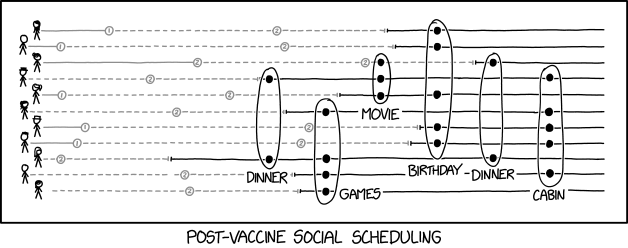
\includegraphics[width=0.8\linewidth]{tex/img/post_vaccine_social_scheduling.png}
	\caption{\emph{As if this problems weren't $\mathcal{NP} $-Hard enough}.
		Post-vaccine social scheduling may be $\mathcal{NP} $-Hard \cite{Munroe}}%
	\label{fig:tex/img/post_vaccine_social_scheduling}
\end{figure}

\paragraph{$\mathcal{NP} $-Complete}%
\label{par:_np_hard} is the set of problems in $\mathcal{NP} $-Hard that are
also in $\mathcal{NP} $. Intuitively these correspond the most difficult
problems to solve in $\mathcal{NP} $. The number of problems which are known to
be in this set is in the order of a thousand \cite{SanjeevArora2017}.

\subsection{$\mathcal{P} $ vs $\mathcal{NP}$}%
\label{sub:_p_vs_np_}

A fundamental question in Computational Complexity is wheter $\mathcal{P} =
	\mathcal{NP} $. Mostly people believe that this is not true, so
$\mathcal{P} \neq \mathcal{NP} $, and also our daily experience tell us that
often it is easier to check the correctness of a solution of a problem than
finding it \cite{9780521884730}: in many cases coming up with the correct
answer requires searching over an exponentially large set
\cite{SanjeevArora2017}. Nonetheless no mathematical proof of this notion has
been found and, in fact, in the last decades there has been little or no progress towards it \cite{Erickson2019}.

If, it is mostly accepted, $\mathcal{P} \neq \mathcal{NP} $ this would produce
a situation as depicted in \autoref{fig:tex/img/complexity-diagram}:
there are problems for which we are not able to find the solution
efficiently (i.e. in polynomial time). On the other side this allows the
existance of one-way-functions (i.e. functions whose inverse is much harder to
compute than the original functions) on which Modern Criptography heavily
relies \cite{9780521884730}.
%
% This brings the need for algorithms which are able to approximate the solution
% in a reasonable amount of time.

% Viceversa, if $\mathcal{P} = \mathcal{NP} $, it would be very easy to find
% proofs and mathematicians could be replaced by
% look at 2.7.3 in Sanjeev's book

\begin{figure}
	\centering
	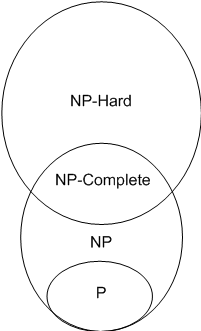
\includegraphics[width=0.3\linewidth]{tex/img/complexity-diagram.png}
	\caption{Venn diagram for the complexity classes if $\mathcal{P} \neq
			\mathcal{NP} $ \cite{article}}%
	\label{fig:tex/img/complexity-diagram}
\end{figure}

\subsection{Optimization Problems and $\mathcal{NPO} $}%
\label{sub:optimization_problems}

Optimization problems are defined from a problem instance $x$, a set of
feasible solutions $S$ and a cost function that takes as input the problem
instance $x$ a feasible solution $s \in S$, denoted as cost$_{O} (x, s) $.
Given a minimization (maximization) problem the optimal solution is defined as
the $s$ minimizing (maximizing) the value of cost$_{O} (x, s)$, and we denote
by opt$_{O} (x) $ this value\cite{Trevisan2004}.

\paragraph{$\mathcal{NPO} $}%
\label{par:_npo_}

is then the set of optimization problems whose cost function
can be computed in polynomial time and for every instance of the problem $x$
and feasible solution for that problem $s \in A$ there is a polynomial $q \; s.t.
	\; s \leq q(|x|)$ (i.e. the size of every solution is bounded by a polynomial
in $x$).

If $\mathcal{P} \neq \mathcal{NP} $ for many optimization problems there is no
algorithm for finding the optimal solution in polynomial time
\cite{Trevisan2004}. This is again a fundamental limitation about what we can
compute which then requires the definition of some alternative approaches, like
the definition of \emph{approximation algorithm}
which are able to be computed in polynomial time
a solution which lies in a given factor from the optimal
one\cite{Vazirani2002}.

\paragraph{Approximation}%
\label{par:r_approximations}

$A$ is an r-approximation algorithm for an $\mathcal{NPO} $ minimization
problem $O$ if, for every instance $x$ of $O$ it holds that
\begin{equation*}
	cost_{O} (x, A(x)) \leq r \cdot opt_{O} (x)
\end{equation*}

\noindent
(or, respectively, cost$_{O} (x, A(x))
	\leq 1/r \cdot $opt$_{O} (x) $ for maximization problems), $A(x)$ being the
optimal solution found by the approximation algorithm \cite{Trevisan2004}.

\subsection{Approximation preserving reductions}%
\label{sub:approximation_preserving_reductions}

Problems approximability varies widely: while for some of them exists
constant factor approximations, for some others even a remotely approximate
solution cannot be found \cite{Ausiello2005} (some examples are listed in
\autoref{tab:inapproximability-examples} ).

% todo: reference to the papers proving each result instead of the hub
\begin{table}
	\centering
	\caption{Examples of known inapproximability results, assuming $\mathcal{P}
			\neq \mathcal{NP} $ \cite{10.1007/3-540-63248-4_10} }
	\label{tab:inapproximability-examples}
	\begin{tabular}{c|p{5cm}|c}
		Problem                                                          & Description                                                   & Inapproximability \\
		\hline
		$ \textsc{MaxClique} $                                           & Biggest complete subgraph                                     & $|V|^{1-
		\epsilon}, \forall \epsilon > 0 $                                                                                                                    \\
		                                                                 &                                                               &                   \\
		$ \textsc{MaximumIndipendentSet} $                               &
		Biggest set of not connected nodes                               & $|V|^{1-
		\epsilon}, \forall \epsilon > 0 $                                                                                                                    \\
		                                                                 &                                                               &                   \\
		$ \textsc{MinCut} $                                              & Partition of nodes in 2 sets $V_1$ and $V_2$ minimizing edges
		between the 2 sets                                               & 1.0624                                                                            \\
		                                                                 &                                                               &                   \\
		$ \textsc{MaximumSetPacking} $                                   & Given a collection of
		finite sets $C$,
		finding the biggest collection $C' \subseteq C$ of disjoint sets & $|C|^{1-
		\epsilon}, \forall \epsilon > 0 $                                                                                                                    \\
	\end{tabular}
\end{table}

\emph{Approximation preserving reductions} are a fundamental notion for proving
a partial order among optimization problems \cite{Ausiello2005}. An
\emph{Approximation preserving reductions} must have
the following properties (when reducing from a problem $A$ to a problem $B$)
\cite{DemaineFall2014}:

\begin{itemize}
	\item any instance $x$ of $A$ should be mapped to an instance $x' = f(x)$
	      of $B$ in polynomial time
	\item any solution $y' \in $ sol$(f(x))$ of $B$ should be associated to a corresponding
	      solution $y = g(x, y') \in $ sol$(x)$ of $A$ in polynomial time
\end{itemize}

So there are 2 efficient (i.e. requiring polynomial time) functions $f$ and $g$
for mapping instances of $A$ to $B$ and solution of $B$ to solutions of $A$,
respectively (\autoref{fig:tex/img/reduction_scheme}).

\begin{figure}
	\centering
	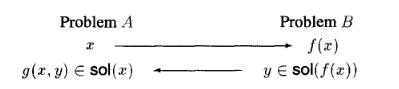
\includegraphics[width=0.6\linewidth]{tex/img/reduction_scheme.png}
	\caption{The reduction scheme \cite{Crescenzi1997ASG}}%
	\label{fig:tex/img/reduction_scheme}
\end{figure}

There are at least 9 different kinds of approximation preserving reductions
\cite{DemaineFall2014}(\autoref{fig:tex/img/approximation_preserving_reductions}) but we will
focus only on one type.

\begin{figure}[b]
	\centering
	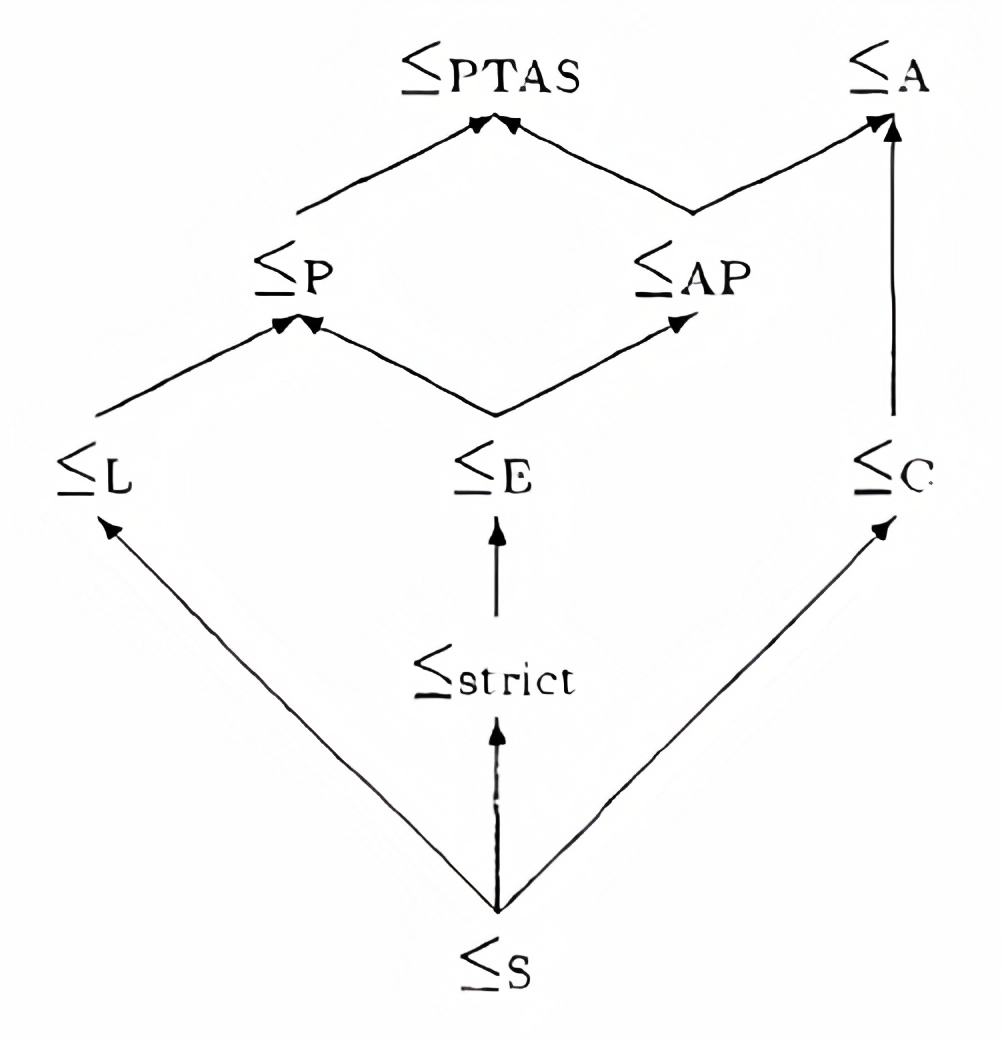
\includegraphics[width=0.4\linewidth]{tex/img/approximation_preserving_reductions.png}
	\caption{Taxonomy of approximation preserving reductions \cite{Crescenzi1997ASG}}%
	\label{fig:tex/img/approximation_preserving_reductions}
\end{figure}

\subsubsection{S reductions}%
\label{sub:strict_reductions}

An $S$ \emph{reduction} from problem $A$ to problem $B$ has the following properties \cite{Crescenzi1997ASG}:
\begin{itemize}
	\item fox any instance $x$ of problem $A$ it holds that opt$_{A} (x) = $ opt$_{B} (f(x))$
	\item for any instance $x$ of $A$ and solution $y'$ of $B$, cost$_{A} (x,
		      g(x, y')) = $ cost$_{B} (f(x), y')$
\end{itemize}

Strict reductions are the strongest type of \emph{approximation preserving
	reductions} and imply all the others \cite{Crescenzi1997ASG}.

\section{Linear and Mixed Integer Programming}%
\label{sec:linear_and_mixed_integer_programming}

\acrlong{LP} is a widely used optimization technique and one of the most
effective; the term refers to problems in which both the constraints and \emph{objective
	function} are linear
\cite{Edgar2001}\cite{Vanderbei2008}\cite{Dantzig1998}\cite{Martin1998}.

\subsection{The structure of a linear programming model}%
\label{sub:the_structure_of_a_linear_programming_model}

In a \acrfull{LP} problem we are given a vector $ \mathbf{c} = (c_1,
	\dots, c_n) $ and we want to maximize (or minimize) a linear function over
the variables $ \mathbf{x} = (x_1, \dots, x_n) $ with the coefficients of the
vector $ \mathbf{c} $, i.e.
\begin{equation*}
	\mathbf{cx} = \sum^{n}_{i=1} c_i x_i
\end{equation*}
(known as the \emph{objective function}) while satisfying some linear
constraints over the variables \cite{Bertsimas1997}\cite{Vanderbei2008}:

\begin{equation*}
	a_1 x_1 + \dots + a_n x_n \begin{Bmatrix} \leq \\ = \\ \geq \end{Bmatrix} b
\end{equation*}

% There is no \emp{a priori} preference regarding how the problem is formulated
% since it is easy to convert an inequality into a equality constraint through
% additional variables ($\omega $ in the example below) called \emph{slack}
% \cite{Vanderbei2008}. For example one in the form
% \begin{equation*}
%     a_1 x_1 + \dots + a_n x_n \leq b
% \end{equation*}
% is equivalent to
% \begin{equation*}
%     a_1 x_1 + \dots + a_n x_n + \omega = b, \quad \omega \geq 0
% \end{equation*}
% and viceversa an equality
% \begin{equation*}
%     a_1 x_1 + \dots + a_n x_n = b
% \end{equation*}
% can be converted into
% \begin{align*}
%     a_1 x_1 + \dots + a_n x_n \leq b \\
%     a_1 x_1 + \dots + a_n x_n \geq b
% \end{align*}
%
In general is possible to formulate any \acrshort{LP} problem as follows (called \emph{standard form}) \cite{Vanderbei2008}

\begin{alignat}{3}
	\label{eq:standard-form}
	\begin{aligned}[t]
		\text{maximize}   &       & \sum_{i=1}^{n} c_{i}x_{i}                                          \\
		\text{subject to} & \quad & \sum_{i=1}^{n} a_{1i}  x_{i} & \leq b_{1} &                        \\
		                  &       & \vdots                                                             \\
		                  &       & \sum_{i=1}^{n} a_{mi}  x_{i} & \leq b_{m} &                        \\
		                  &       & x_{i}                        & \geq 0,    & \quad i & =1 ,\dots, n
	\end{aligned}
\end{alignat}


The $x_i$ are known also as \emph{decision variables}; a choice of $ \mathbf{x}
$ if called \emph{solution} and \emph{feasible solution} if it satisfies the
constraints, \emph{optimum} if it maximizes the \emph{objective function}
\cite{Vanderbei2008}.

\subsection{Solving an LP problem}%
\label{sub:solving_an_lp_problem}

Solving an \acrshort{LP} problem involves a process called the \emph{simplex
	method} which has 2 different phases.

Starting from the \emph{standard form} (\autoref{eq:standard-form})
\emph{slack} variables $x_{n+1}, \dots, $ $x_{n+m} $ are introduced as well as a name
for the \emph{objective} function, allowing to express the problem as follows
\cite{Vanderbei2008}\cite{Edgar2001}

\begin{alignat}{2}
	\label{eq:standard-form}
	 &  & \quad &
	\begin{aligned}[t]
		\zeta   & = \sum_{i=1}^{n} c_{i}x_{i}                                       \\
		x_{n+1} & = b_{1} - \sum_{i=1}^{n} a_{1i}  x_{i} &                          \\
		\vdots                                                                      \\
		x_{n+m} & = b_{m} - \sum_{i=1}^{n} a_{mi}  x_{i} &                          \\
		x_{i}   & \geq 0,                                & \quad i & =1 ,\dots, n+m
	\end{aligned}
\end{alignat}

The first phase involves finding a feasible solution for the problem. More
specifically, we look for $m$ variables, called \emph{basic variables}, whose
value we choose in order to satisfy the $m$ equality constraints (while the
remaining variables, the \emph{nonbasic} ones, are set to 0); if no such
feasible solution exists then the problem is \emph{unfeasible}. Let $\mathcal{B}
$ be the set of \emph{basic variables} and $\mathcal{N} $ the set of
\emph{nonbasic variables} \cite{Vanderbei2008}\cite{Bertsimas1997}. Then the
problem can be reformulated as follows

\begin{alignat}{2}
	\label{eq:standard-form-simplex-new}
	 &  & \quad &
	\begin{aligned}[t]
		\zeta & = \bar{\zeta} + \sum_{j \in \mathcal{N} }^{n} c_{j}x_{j}                                      \\
		x_{i} & = \bar{b}_{i} - \sum_{j \in \mathcal{N} }^{n} \bar{a}_{ij}
		x_{j} & i                                                          & \in \mathcal{B}                  \\
		x_{i} & \geq 0,                                                    & \quad i         & =1 ,\dots, n+m
	\end{aligned}
\end{alignat}

The second phase of the \emph{simplex method} aims at improving the current
solution: if $c_{j} \geq 0, \; \forall j \in \mathcal{N} $ then the value of the
objective function cannot be increased and we found an optimum. If, instead, there is at least a $c_{j}
	> 0$ then we can increase the value of $\zeta$ by increasing $x_{j} $; now
there are 2 different cases \cite{Vanderbei2008}
\begin{itemize}
	\item as $x_{j} $ increases there is at least a variable $\tilde{x}_{j} $
	      whose value needs to decrease to satisfy equality constraints. The first
	      of these variables $\tilde{x}_{j} $ reaching to $0$ moves from
	      $\mathcal{B} $ to $\mathcal{N} $, while
	      $x_{j} $ moves from $\mathcal{N} $ to $\mathcal{B} $. The problem is reformulated again as in
	      \autoref{eq:standard-form-simplex-new} and the process is repeated
	      \cite{Vanderbei2008}.
	\item if no such $\tilde{x}_{j} $ variable exists then the value of $x_{j}
	      $ can be increased indefinitely and the problem is said to be
	      \emph{unbounded}, i.e. it can achieve any arbitrarily large value.
\end{itemize}

The process is illustrated in \autoref{fig:tex/img/simplex}.

\begin{figure}
	\centering
	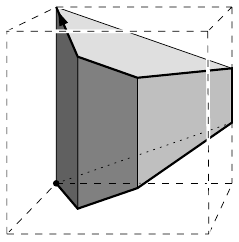
\includegraphics[width=0.4\linewidth]{tex/img/simplex.png}
	\caption{An example of the progress of the \emph{simplex method}: the
		process moves along the vertices of the polygon defined by the
		contraints while improving the value of the solution \cite{BerndGaertner2006}}%
	\label{fig:tex/img/simplex}
\end{figure}

\subsection{Mixed Integer Programming}%
\label{sub:mixed_integer_programming}

Many problems involve not only continous variables but also variable that take binary or
integer values: these are known as \acrfull{MIP} problems. Furthermore, some of
these problems are linear in the constraints and objective function and are
known as \acrfull{MILP} problems
\cite{Edgar2001}\cite{Wolsey1998}.

A generic \acrshort{MILP} can be expressed as \cite{Conforti2016}

\begin{alignat}{3}
	\label{eq:standard-form-milp}
	\begin{aligned}[t]
		\text{maximize}   &                                     & \sum_{i=1}^{n_{1} } c_{i}x_{i} +
		\sum_{i=1}^{n_{2} } h_{i}y_{i}                                                                                                                               \\
		\text{subject to} & \quad                               & \sum_{i=1}^{n_{1} } a_{1i}  x_{i} + \sum_{i=1}^{n_{2} } g_{1i}  y_{i} & \leq b_{1}       &         \\
		                  &                                     & \vdots                                                                                             \\
		                  &                                     & \sum_{i=1}^{n_{1} } a_{mi}  x_{i} + \sum_{i=1}^{n_{2} } g_{1i}  y_{i} & \leq b_{m}       &         \\
		% &       & \sum_{i=1}^{n} a_{mi}  x_{i}                                          & \leq b_{m} &                        \\
		                  &                                     & x_{i}
		                  & \geq 0,                             & \quad i                                                               & =1 ,\dots, n_{1}           \\
		                  &                                     & y_{i}                                                                 & \geq 0,          & \quad i
		                  & =1 ,\dots, n_{2} \; \text{integral}
	\end{aligned}
\end{alignat}

For convenience we will refer to \acrshort{MILP} problems as \acrshort{MIP} in
the rest of the document.

The \emph{relaxation} of a \acrshort{MIP} problem is defined as the same
problem where the integrality constraints have been removed \cite{Edgar2001}.

Solving a \acrshort{MILP} is a difficult task in general, differently from the
\acrshort{LP} problems. It has been shown also that \acrshort{MIP} is
$\mathcal{NP}$-\textbf{Hard}
\cite{Kannan1978}\cite{Liberti2019}\cite{Schrijver1998}. This is why the \emph{relaxation} is often considered
to get an approximation of the exact solution and it is much easier
\cite{Conforti2016}.

\subsection{Solving a MIP}%
\label{sub:solving_a_mip}

One approach that has been proven successfull for solving \acrshort{MIP} is th
e Branch-and-Bound, which is guaranteed to find an optimal solution
\cite{Conforti2016}\cite{Edgar2001}.

Given a problem $P$ the process starts by solving the \emph{relaxation} of $P$
and finding its optimal solution $(\tilde{x}, \tilde{y})$.
Let $S$ and  $\tilde{S}$ be the set of feasible solutions
for the original problem $A$ and its relaxation, respectively. By definition
we have that $S \subseteq \tilde{S} $.
Therefore \cite{Edgar2001}
\begin{itemize}
	\item If the relaxation problem is not feasible so will also the original
	      problem
	\item If $\tilde{y}$ has only integer values then we found the optimal
	      solution for the original problem $A$
\end{itemize}

If, instead, $\tilde{y}$ contains some fractional values, we start by
initialing the value of the best solution so far, $\zeta$, with $-\infty$.
Then we choose one of the fractional variables that are required to be integral
in the original problem $A$, say $y_j$ with value $f$, and create $2$
subproblems, respectively adding the constraint $y_{j} \leq \lfloor f \rfloor$
and $y_{j} \geq \lceil f \rceil$. This step is called \emph{branching}. We now
consider the solution of each subproblem $(x_j, y_j)$ with value of the
objective function $z_{j} $ \cite{Edgar2001}\cite{Conforti2016}.

\begin{itemize}
	\item If either of the subproblems is not feasible or its value $z_{j} $ is
	      lower then the best one found so far then it does not to be
	      considered further. This is called \emph{pruning}.
	\item otherwise if $y_{j} $ are all integer values then $\zeta = z_{j} $
	\item otherwise we subdivide again in $2$ subproblems as done above.
\end{itemize}

When there are no remaining subproblems to consider the Branch-and-Bound method
terminates \cite{Edgar2001}.
